\documentclass[titlepage]{tufte-book}

\usepackage[runall=true]{pythontex}
\setpythontexworkingdir{<outputdir>}
\usepackage{environ}
\usepackage{morewrites}
\usepackage{amsthm}
\usepackage{amsmath}
\usepackage{amssymb}
\usepackage[pdftex]{graphicx}
\usepackage{epstopdf}
\usepackage{hyperref}
\usepackage{alltt}
\usepackage{listings}
\usepackage{array}
\usepackage{extarrows}
\usepackage{setspace}
\usepackage{tikz}
\usepackage{tikz-qtree}
\usetikzlibrary{calc}
\usetikzlibrary{positioning}
\usepackage{hyperref}
\usepackage{graphviz}
\usepackage{geometry}                % See geometry.pdf to learn the layout options. There are lots.
\usepackage{bashful}
\usepackage{microtype} % Improves character and word spacing
\usepackage{caption}

\usepackage{booktabs} % Better horizontal rules in tables

\setkeys{Gin}{width=\linewidth,totalheight=\textheight,keepaspectratio} % Improves figure scaling
\graphicspath{{figures/}}

\usepackage{fancyvrb} % Allows customization of verbatim environments
\fvset{fontsize=\normalsize} % The font size of all verbatim text can be changed here

\newcounter{problem}
\newcounter{total}
\newcommand{\step}[1]{{}
\vspace{4pt} \noindent {\bf \theproblem. }#1\addtocounter{problem}{1}}

\newcommand{\cut}[1]{}

\usepackage[tikz]{bclogo}
\usepackage{tikz}
\usetikzlibrary{calc}

\lstdefinestyle{BashInputStyle}{
  language=bash,
  basicstyle=\small\ttfamily,
  numberstyle=\tiny,
  showstringspaces=false,
  numbersep=3pt,
  otherkeywords={|, ;, ', ", *,>, <, *, &, `, $},
  alsoletter={:~_},
  columns=fullflexible,
  backgroundcolor=\color{yellow!20},
  linewidth=0.93\linewidth,
  xleftmargin=0.03\linewidth,
  keywordstyle=\color{blue},
  emph={ls, cat, head, tail, more, less, sort, uniq, kill java, grep, zip, unzip, tar, wc, cp, chmod,chown},
  emphstyle=\color{black}\bfseries,
    commentstyle=\color{gray}\slshape
    }

\newcommand{\chili}{\scalebox{.04}{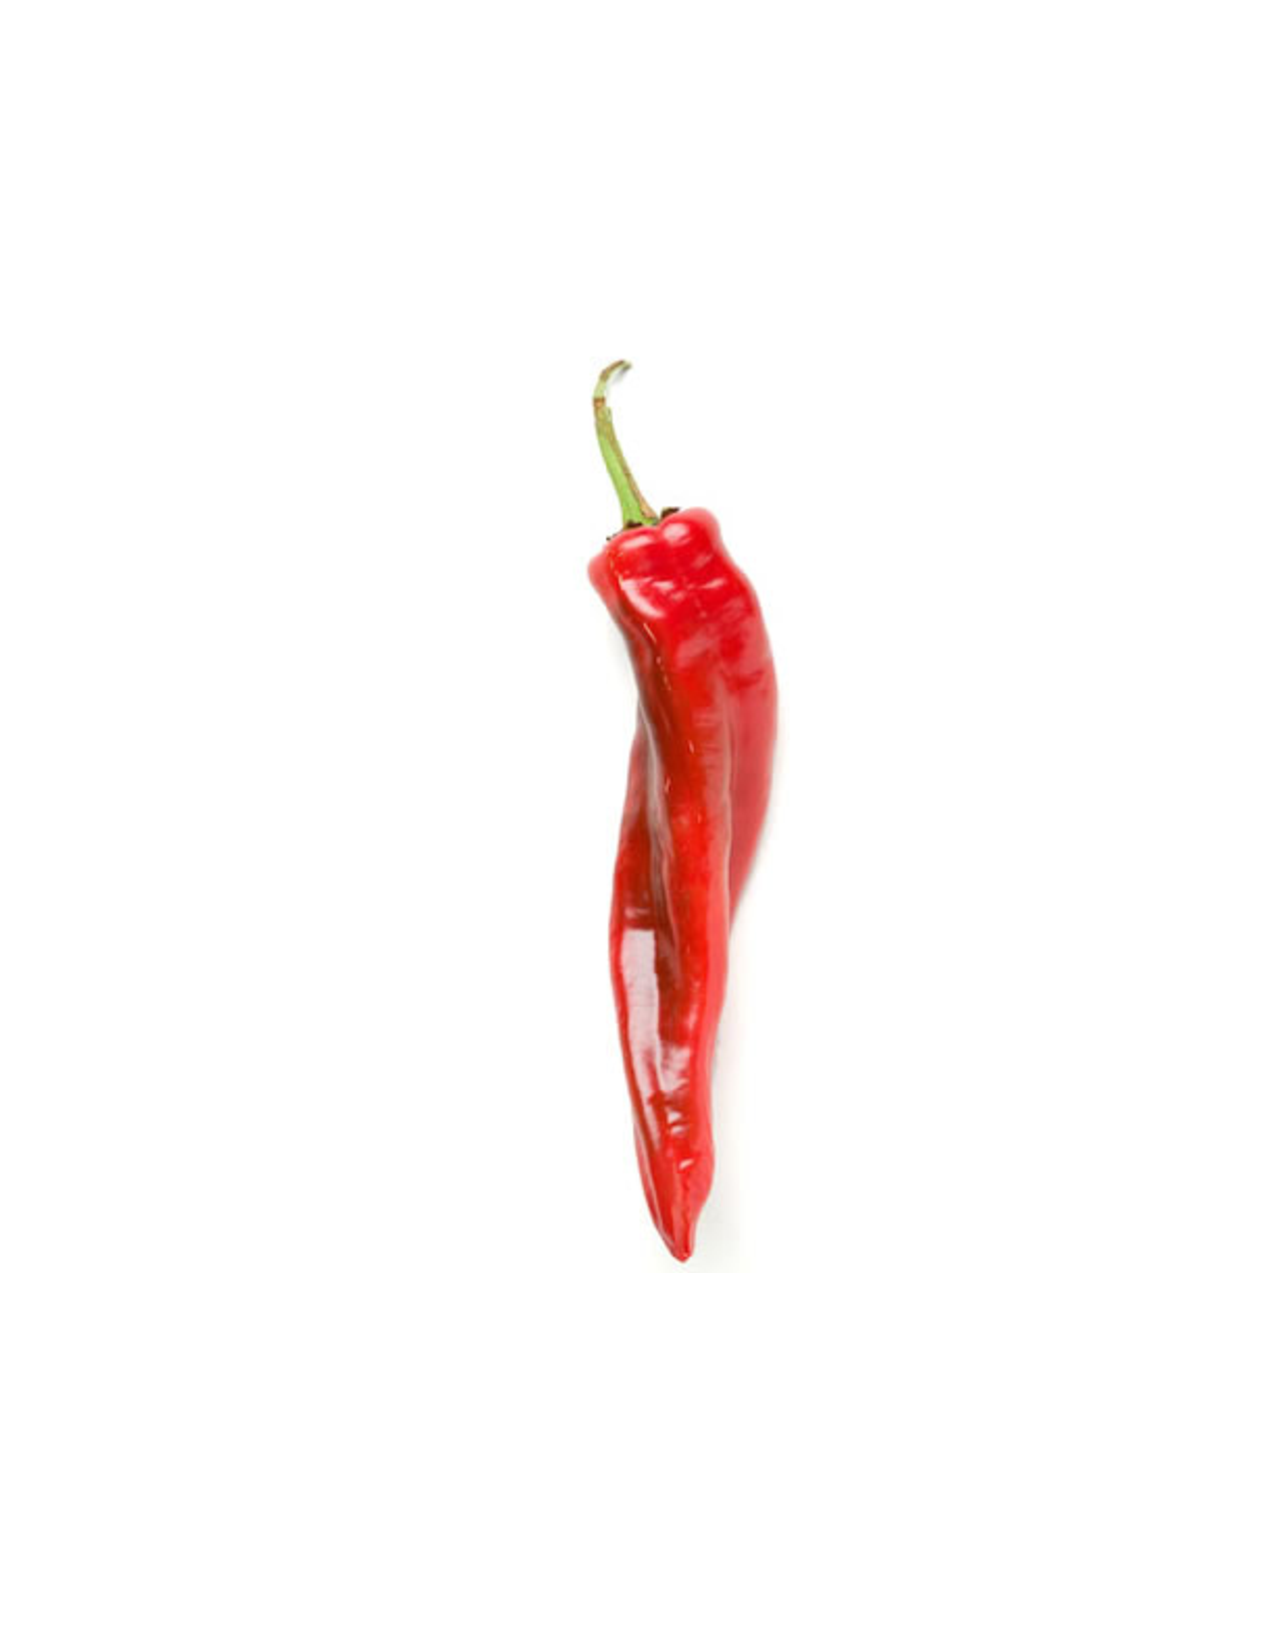
\includegraphics{figures/chili.pdf}}}
\newcommand{\chchili}{{\chili\chili}}
\newcommand{\chchchili}{{\chchili\chili}}

% The units package provides nice, non-stacked fractions and better spacing
% for units.
\usepackage{units}

% The fancyvrb package lets us customize the formatting of verbatim
% environments.  We use a slightly smaller font.
\usepackage{fancyvrb}
\fvset{fontsize=\normalsize}

% Small sections of multiple columns
\usepackage{multicol}

\hypersetup{
urlcolor=blue,
colorlinks=true
}
\usepackage[noline, procnumbered, linesnumberedhidden, boxed]{algorithm2e}

\newcommand{\openepigraph}[2]{ % This block sets up a command for printing an epigraph with 2 arguments - the quote and the author
\begin{fullwidth}
\sffamily\large
\begin{doublespace}
\noindent\allcaps{#1}\\ % The quote
\noindent\allcaps{#2} % The author
\end{doublespace}
\end{fullwidth}
}

\newcommand{\figref}[1]{Figure~\ref{#1}}
\renewcommand{\thefigure}{\arabic{figure}}

\newenvironment{callout}[1]{
\[
  \left[
      \begin{tabular}{@{\quad}m{.05\textwidth}@{\qquad}m{.75\textwidth}@{\quad}}
        \scalebox{1.5}{#1} & 
          \raggedright%
}
{
      \end{tabular}
    \right]
\]
}

\newcommand{\blankpage}{\newpage\hbox{}\thispagestyle{empty}\newpage} % Command to insert a blank page

\usepackage{makeidx} % Used to generate the index
\makeindex % Generate the index which is printed at the end of the document

\renewcommand{\maketitlepage}[0]{%
  \cleardoublepage%
  {%
  \sffamily%
  \begin{fullwidth}%
  ~
  \vspace{11.5pc}%
  \fontsize{36}{40}\selectfont\par\noindent\textcolor{darkgray}{\allcaps{\thanklesstitle}}%
  
\scalebox{.2}{
\includegraphics{figures/msan-logo}}
  \vspace{11.5pc}%
  \fontsize{12}{18}\selectfont\par\indent\textcolor{darkgray}{\allcaps{\thanklessauthor}\\
\indent{\tt parrt@cs.usfca.edu}\\
\href{http://parrt.cs.usfca.edu}{http://parrt.cs.usfca.edu}}%
  \vspace{11.5pc}%
  \fontsize{14}{16}\selectfont\par\noindent\allcaps{\thanklesspublisher}%
  \end{fullwidth}%
  }
  \thispagestyle{empty}%
  \clearpage%
}

\titlecontents{part}% FIXME
    [0em] % distance from left margin
    {\vspace{1.5\baselineskip}\begin{fullwidth}\LARGE\rmfamily\itshape} % above (global formatting of entry)
    {\contentslabel{2em}} % before w/label (label = ``II'')
    {} % before w/o label
    {\rmfamily\upshape\qquad\thecontentspage} % filler + page (leaders and page num)
    [\end{fullwidth}] % after

  \titlecontents{chapter}%
    [0em] % distance from left margin
    {\vspace{1.5\baselineskip}\begin{fullwidth}\Large\rmfamily\itshape} % above (global formatting of entry)
    {\hspace*{0em}\contentslabel{2em}} % before w/label (label = ``2'')
    {\hspace*{4em}} % before w/o label
    {\rmfamily\upshape\qquad\thecontentspage} % filler + page (leaders and page num)
    [\end{fullwidth}] % after

\titlespacing*{\chapter}{0pt}{0pt}{30pt}
\titlespacing*{\section}{0pt}{3.5ex plus 1ex minus .2ex}{2.3ex plus .2ex}
\titlespacing*{\subsection}{0pt}{3.25ex plus 1ex minus .2ex}{1.5ex plus.2ex}

\begin{document}


\chapter{The Central Limit Theorem in Action}

\setcounter{problem}{1}

\section{Goal}

\begin{fullwidth}

You are studying the central limit theorem in the statistics boot camp or have seen it before. Our goal is to observe the central limit theorem in action whereby the means of samples drawn from a uniform random variable follow a normal distribution.

\section{Discussion}

Statistical inference is all about estimating statistics about a population from a sample or samples. The {\em central limit theorem} (CLT) is a critical piece of the machinery that allows us to infer things about a population. 

In a nutshell, the CLT says that if we look at the sample means for a bunch of samples drawn from some distribution with mean $\mu$ and variance $\sigma^2$, the means will bounce around the true population mean.  That means that the sample mean is  itself a random variable and the CLT tells us the distribution is $N(\mu, \sigma^2/n)$ for sample size $n$.  Things to note:

\begin{enumerate}
\item $X$'s distribution doesn't really matter (that's close enough to the truth for our purposes)---the distribution of its sample mean is normal. 

\item The variance of the sample mean (not the sample variance), $\sigma^2/n$, gets tighter as we increase the sample size $n$.

\item More trials (number of $X$ samples we conjure up) improves the resolution of the sample-mean normal distribution but doesn't change the variance. In other words,  more samples help our visualization of the sample mean distribution but it does not change our estimate of the sample mean.
\end{enumerate}

\noindent We are going to observe the sample mean distribution for a uniform random variable in $U(a=0,b=1)$ with $\mu=\frac{a+b}{2}=0.5$ and $\sigma^2 = \frac{(b-a)^2}{12}=\frac{1}{12}$.  The histogram should therefore show normal distribution $N(0.5,(1/12n))$ for sample size $n$.


\subsection{Steps}

The complete code is in \href{https://github.com/parrt/msan501/blob/master/notes/code/clt.py}{\textcolor{blue}{\tt notes/code/clt.py}} but here are the key steps.

\step Get TRIALS=500 samples $X$ of size $n=4=LEN(X)$ from the uniform distribution $U(0,1)$ using our {\tt runif01()} function or Python's {\tt random.random()}.  Compute the mean of each $X$ vector and add it to the end of a different array {\tt X\_}.

\step Plot the histogram of {\tt X\_} with {\tt bins=60, normed=1}.  

\step Let's add the theoretical normal distribution on top. To do that we need the appropriate parameters of $N(\mu, \sigma^2/n)$. The mean  $\mu$ of uniform samples should be midway between $a$ and $b$ from $U(a,b)$. In our case, that's 0.5 since we are doing $U(0,1)$. The variance of the uniform distribution is $(b-a)^2/12$ and we need the variance divided by sample size $n$.   We can define a function that returns the variance of uniform distribution $U(a,b)$:

\begin{pyverbatim}
def unifvar(a, b):
	return ((b - a) ** 2) / 12.0
\end{pyverbatim}

\step  To get the theoretical distribution, let's define it ourselves from

\[
P(x) = \frac{1}{{\sigma \sqrt {2\pi } }}e^{{{ - \left( {x - \mu } \right)^2 } \mathord{\left/ {\vphantom {{ - \left( {x - \mu } \right)^2 } {2\sigma ^2 }}} \right. \kern-\nulldelimiterspace} {2\sigma ^2 }}}
\]

\begin{pyverbatim}
def normpdf(x, mu, sigma): # sigma is the standard deviation, sigma^2 is the variance
    """
    Accept either a floating-point number or a numpy ndarray, such as what you get
    from arange().  You do not need a loop in the code does not change here
    because 2 * ndarray is another ndarray automatically. In this respect,
    numpy is very convenient and behaves like R.
    """
    u = - (x - mu)**2 / (abs(sigma)**2 * 2.0)
    y = (1.0 / (math.sqrt(2 * math.pi) * abs(sigma))) * math.e ** u
    return y
\end{pyverbatim}

\step Then, plot the theoretical normal distribution on top of the histogram. (Also set the axes so that we can use the same range throughout the next series of tests to see how the distribution changes.) Note that the usual normal density function provided above expects the {\bf standard deviation not the variance} and so we need to pass {\tt normpdf()} the square root of the expected variance. 

\step Now, display some important parameters in the graph using {\tt text()}. You will need to do the {\tt ax = fig.add\_subplot(111)} thing early in your script. The text in between the \$ symbols is latex and lets us display nice math symbols (e.g., the title), although I'm not doing much with it here.

\begin{pyverbatim}
plt.text(.02, .9, '$N = %d$' % N, transform=ax.transAxes)
plt.text(.02, .85, '$TRIALS = %d$' % TRIALS, transform=ax.transAxes)
plt.text(.02, .8, 'Obs. mean($\\overline{X}$) = %5.5f' % np.mean(X_), transform=ax.transAxes)
plt.text(.02, .75, 'Obs. var($\\overline{X}$) = %5.5f' % np.var(X_), transform=ax.transAxes)
plt.text(.02, .68, 'Obs. $\sqrt{var(\\overline{X})}$ = %3.3f' % np.sqrt(np.var(X_)), transform=ax.transAxes)
plt.text(.02, .63, 'stddev U($0,1$)/%d = %3.3f' % (N, np.sqrt(sample_mean_var)), transform=ax.transAxes)

plt.title("CLT Density Demo. sample mean of U(0,1) is $N(.5, \sigma^2/N)$")
plt.xlabel("$\\overline{X}$", fontsize=16)
plt.ylabel("Density", fontsize=16)
\end{pyverbatim}

\step Run it. The resulting graph should look like this \\

\scalebox{.45}{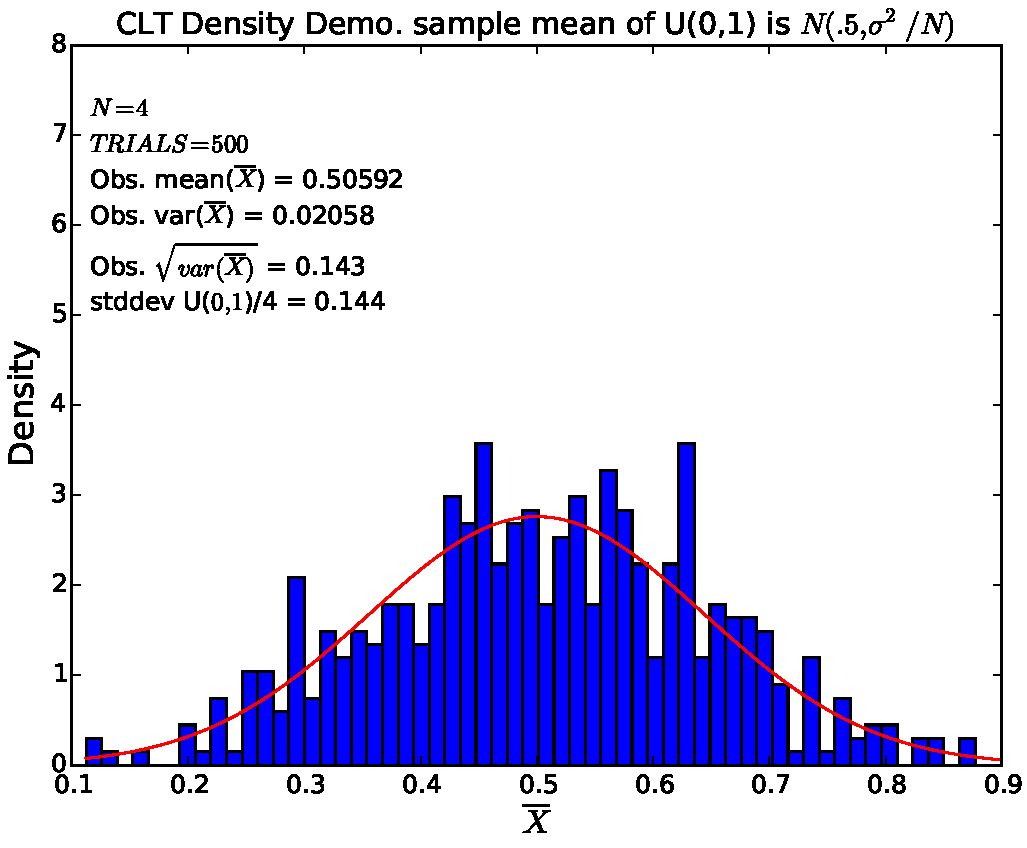
\includegraphics{figures/clt-500-4.pdf}}

\noindent Notice how the mean is close to the expected 0.5 and that the observed stddev of the sample means is close to the theoretical stddev.

\step Increasing the number of trials to 15,000 shows much higher resolution but does not change the variance/tightness of the distribution at all:

\scalebox{.45}{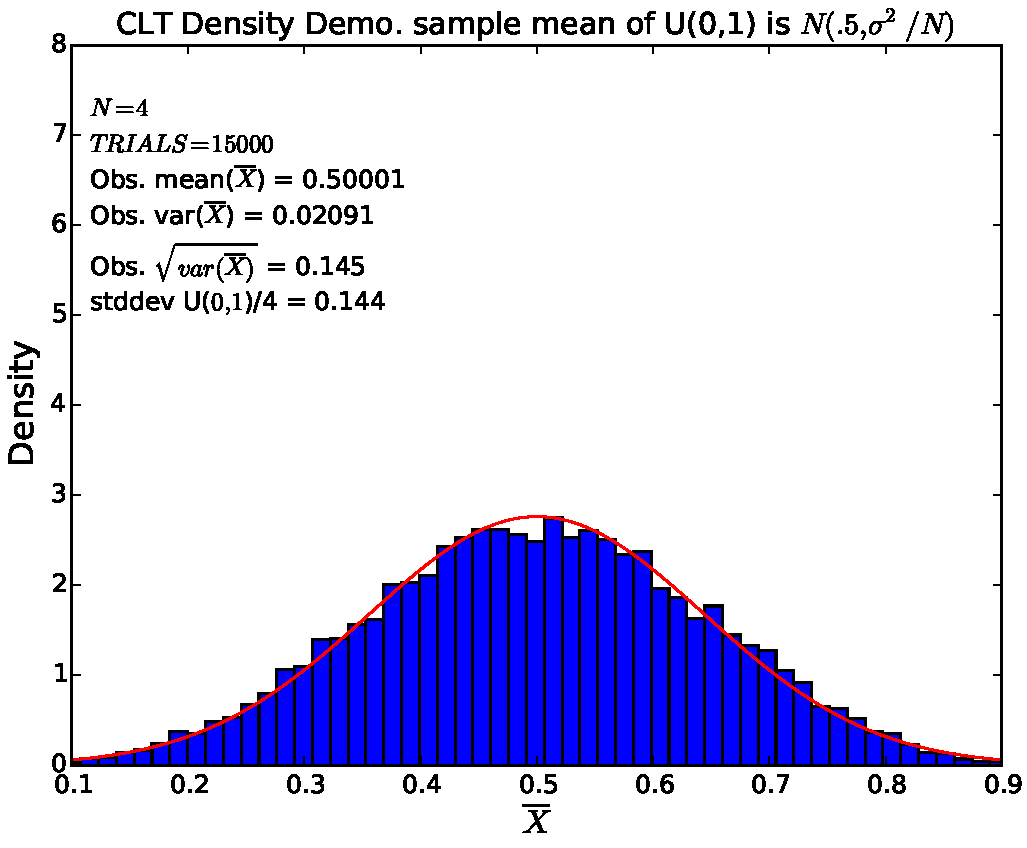
\includegraphics{figures/clt-15000-4.pdf}}

\step Now, if we increase the sample size to $N=20$, we get a much tighter variance on the mean of $\overline{X}$. Run it:

\scalebox{.45}{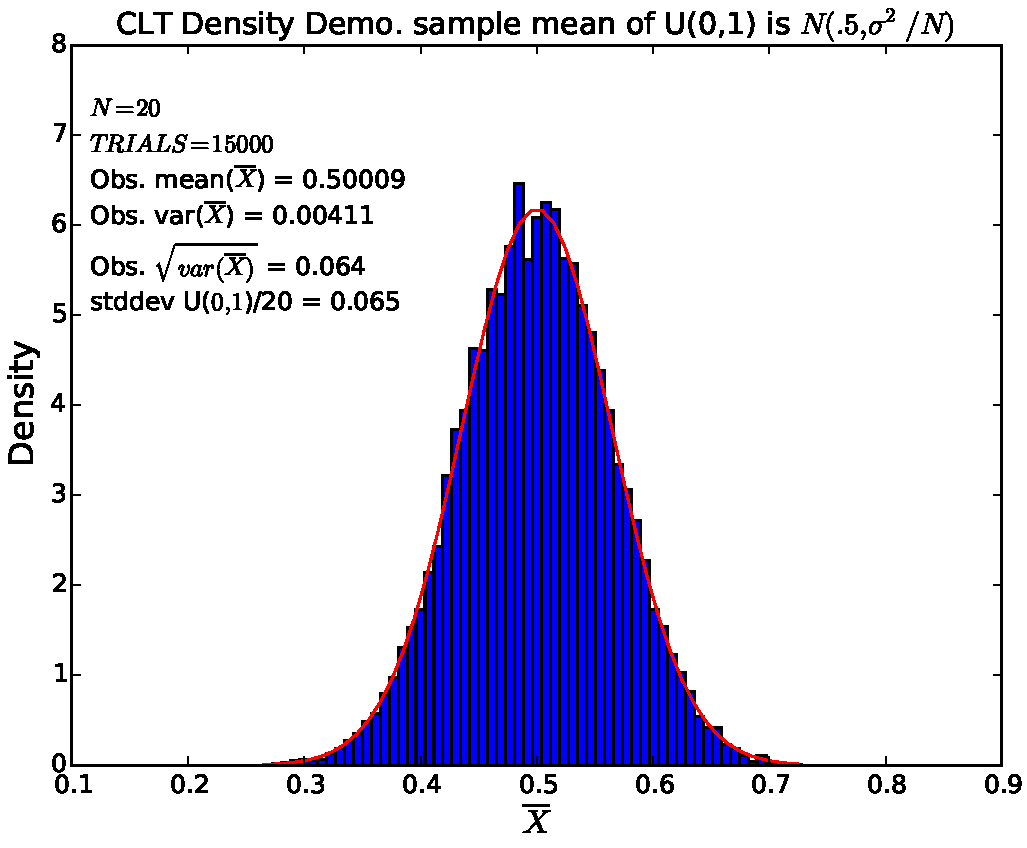
\includegraphics{figures/clt-15000-20.pdf}}

\step Increasing to 40 we get:

\scalebox{.45}{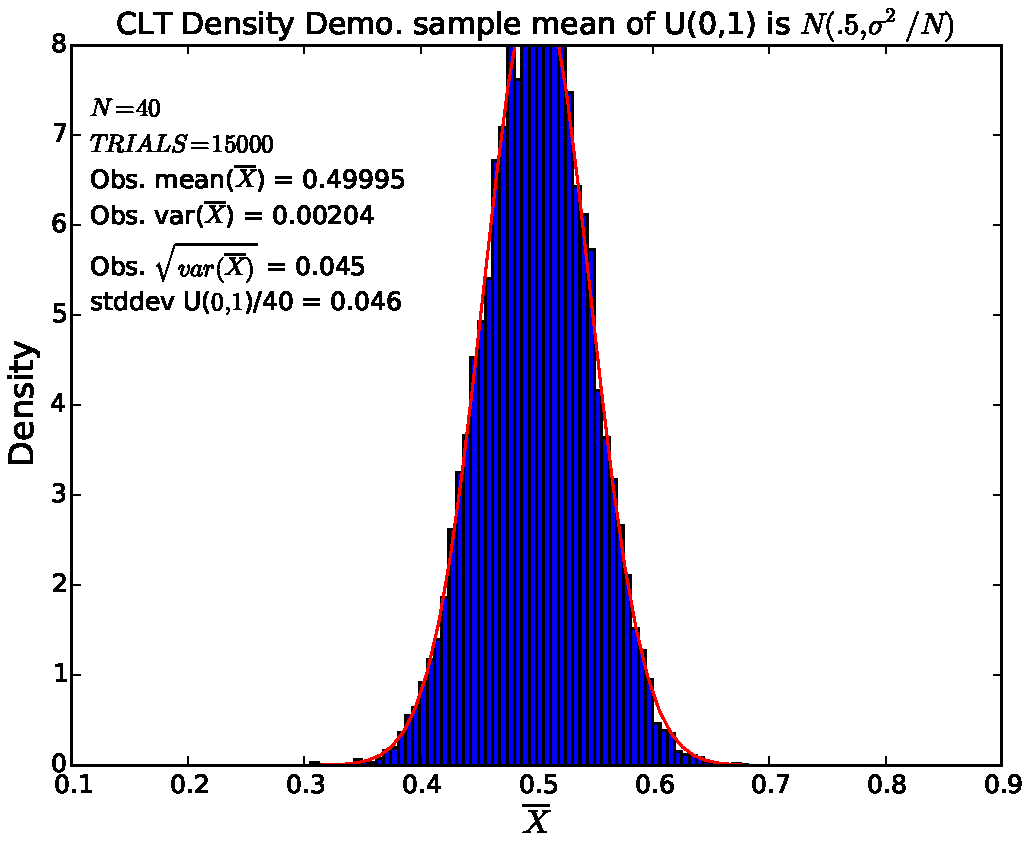
\includegraphics{figures/clt-15000-40.pdf}}

\end{fullwidth}

\end{document}
